

\section{PDMPs and generators} \label{pdmpgenerator}
The main class of stochastic processes utilized in this thesis is the piecewise deterministic Markov Process, or PDMP, whose theory is presented in Davis \cite{dav84}.  For a PDMP, a Markov process is allowed deterministic drift along flow lines of a vector field before randomly jumping to a new state.  In addition to covering several examples from queueing theory, including the  M/G/1 queue, the GI/G/1 queue, the model also encapsulates Markov chains.  Our chief object of interest is the infinitesimal generator and martingale from Dynkin's formula associated with the PDMP.   In Chatpers 3 and 4 we plan to use these martingales to provide an approximation to limiting kinetic equations. 


Our goal is to describe a generalized jump process that takes place on a disjoint union of  manifolds, and follows a deterministic drift between jumps. To characterize the state space, we let $\mathcal S$ be a countable set,   $d:\mathcal S\rightarrow \mathbb{N}$ , where for each $\mathbf s \in \mathcal S$,  $M_\mathbf s \subset \mathbb{R}^{d(\mathbf s)}$ is an open set.   The state space is then the disjoint union
\begin{equation}
E =\coprod_{\mathbf s \in \mathcal S} M_\mathbf s = \left\{(\mathbf s, \textbf x):\mathbf s \in \mathcal S,  \textbf x \in M_\mathbf s \subset \mathbb R^{d(\mathbf s)}\right\}. \end{equation}
To define the topology of $E$, let $\iota_\mathbf s:M_\mathbf s \rightarrow E$ be the canonical injection defined by $\iota_\mathbf s(\textbf{x}) = (\mathbf s, \textbf{x})$.  A set $A$ in $E$ is open if for every $\mathbf s$, $\iota_\mathbf s^{-1}(A)$ is open in $M_\mathbf s$. We then define $\mathcal E$ as the Borel sets of $E$. This makes $(E,\mathcal E)$ a Borel space.  

We now define a stochastic process $X(t) = (\mathbf s(t),\zeta(t))$, with a law $(X(t))_{t  \ge 0}$ based on the following:

\begin{enumerate}
\item 
Vector fields $\mathcal X_\mathbf s,\mathbf s \in \mathcal S.$ defined on $M_\textbf s$.
\item
A measurable function $\lambda:E \rightarrow \mathbb R^+$.
\item
A transition measure $Q: \mathcal E \times (E \cup \Gamma^*) \rightarrow [0,1]$.

\end{enumerate}  

We will formally define $\Gamma^*$, the exit boundary of a PDMP, shortly. To see how this fits in with a generalized jump process, points in $M_{\textbf s}$ will travel according to flows defined by $\mathcal X_\mathbf s$ until either a Poisson clock with intensity $\lambda$ rings, or the point hits the boundary of $M_\mathbf s$. When such an event occurs, the point jumps to a new position in $E$, determined by $Q$.   

The vector fields $\mathcal X_\mathbf s$ are chosen so that for every $z \in M_\mathbf s$, there is a unique integral curve $\phi_\mathbf s(t,z)$ satisfying 
\begin{eqnarray}
 \frac d{dt}f(\phi_\mathbf s(t,z)) = \mathcal X _{\mathbf s}f(\phi_\mathbf s(t,z))\\
 \mathbf \phi_\mathbf s(0,z) =  z \nonumber 
\end{eqnarray}
for any smooth function $f: \mathbb{R}^{d(\mathbf s)} \rightarrow \mathbb{R}$.  Here we also require that the vector fields are conservative, meaning that there exists a $t>0$ where $\phi_\mathbf s(r,z)$ is defined for $r \in [0,t]$.   

 Now let $\partial^*M_\mathbf s$ be the exit boundary of $M_\mathbf s$, defined as
  \begin{equation}
 \partial^*M_\mathbf s =\left \{y \in \partial M_\mathbf s: \phi_\mathbf s(t^-, \textbf{x}) = y \quad \hbox{ for some } (t, \textbf{x}) \in \mathbb{R}_+ \times M_\mathbf s\right \}
\end{equation}
 $\Gamma^*$ is then defined as the exit boundary of our state space:
\begin{equation}
\Gamma^* = \coprod_{\mathbf s \in \mathcal S} \partial ^{*}M_\mathbf s 
\end{equation}
At a given state $\mathbf x \in E$, we define the exit time as 
\begin{equation}
t^*(\mathbf x) = \inf \{t >0: \phi_\mathbf s(t, \textbf{x}) \in \partial ^{*}M_\mathbf s\}.  
\end{equation}
The stochastic process $(X(t))_{t \ge 0}$ with initial condition $X(0) =  (\mathbf s,z)$ is then defined as follows.  For $\mathbf x = (\mathbf s, z)$, define a survivor function $\mathcal F$ as 
\begin{equation}
\mathcal F_{\mathbf x}(t) = \begin{cases} \exp\left(-\int_0^t \lambda(\mathbf s,\phi_\mathbf s(r,z))dr\right), & t<t^*(\textbf{x}), \\ 0, & t \ge t^*(\textbf{x}).
\end{cases} 
\end{equation}
The rate \ $\lambda:E \rightarrow \mathbb R^+$ is a measurable function, where for every state $\textbf{x} = (\mathbf s,  \textbf{x}) \in E$ there exists $\varepsilon > 0$ where the function $s \rightarrow \lambda(\mathbf s, \phi_\mathbf s(s, \textbf{x}))$ is integrable for $s \in [0,\varepsilon)$.  We also define $Q(A;\textbf{x})$ to be a measurable function of $\textbf{x}$ for each fixed $A \in \mathcal E$ on $\textbf{x} \in E \cup \Gamma^*$, and a probability measure on $(E, \mathcal E)$ for each $X \in E \cup \Gamma^*$.


Now choose a random variable $T_1$ such that $\mathbb{P}[T_1>t] = \mathcal F_\mathbf x(t)$.  Now independently choose an $E$-valued random variable $(L,Z)$ with distribution $Q(\cdot ; \phi_\mathbf s(T_1,z))$.  The trajectory of $X(t)$ for $t \le T_1$ is then
\begin{equation}
X(t) = \begin{cases} (\mathbf s,\phi_\mathbf s(t,z)), & t<T_1 \\
(L,Z), & t = T_1.
\end{cases}
\end{equation}
From $X(T_1)$, we choose the next inter-jump time $T_2-T_1$ and $X(T_2)$ in a similar fashion. It can be shown that the process $X(t)$ is Markov, and in fact, strong Markov (Section 3 of \cite{dav84}).  

As a Markov process, the PDMP has an associated infinitesimal generator $\mathcal A$, acting on a domain $\mathcal D(\mathcal A)$, defined as the set of functions $f:E\rightarrow \mathbb R$ where the limit 
\begin{equation}
 (\mathcal Af)(\mathbf x)=  \lim_{t\rightarrow 0^+} \frac{\mathbb E^\mathbf x (f(X(t)))-f(\mathbf x)}{t}
\end{equation}
exists for all $\mathbf x \in E$. The infinitesimal generator then takes the form

\begin{equation}\label{generator}
\mathcal Af(\mathbf x) = \mathcal X(f(\mathbf x))   +\lambda(\mathbf x)\int_E (f(y)-f(\mathbf x))Q(dy;\mathbf x)), \quad f \in \mathcal D(\mathcal A).
\end{equation}
From here, we can use Dynkin's formula to derive the  
martingale
\begin{equation}\label{martingale}
M_t^f := f(X(t)) - f(X(0))-\int_0^t \mathcal A f(X(s))ds,\quad f \in \mathcal D(\mathcal A).
\end{equation}

The following set of sufficient conditions for membership in $\mathcal D(\mathcal A)$ is given in Rolski et. al. \cite{rolski2009stochastic}
\begin{theorem}\label{fourcond} A function $f: E \rightarrow \mathbb{R}$ satisfies $f \in \mathcal D(\mathcal A)$ if the following hold:
  
\begin{enumerate}
\item 
The function $t \rightarrow f(\phi(x,t))$ is absolutely continuous on $[0,s^*(x))$ for every $\mathbf x \in E$, where $s^*(x) = \inf_t\{t|\mathcal F(t) =0\}$. \item
$f(x)  = \lim_{t \rightarrow 0} f(\phi(x,t))$ exists for all $x \in  \Gamma^*$ \item
(Boundary condition):$f(x)= \int_E f(y) Q(dy,x)$ for $x \in \Gamma^*$\item
(Finite expectation of number of jumps): for all $t \in \mathbb{R}^+, x\in E$,
\begin{equation} 
\mathbb{E}\left[\sum_{i = 1}^{m(t)} |f(X(T_i)-f(X(T_{i-1}))|\right]<\infty
\end{equation}
\end{enumerate}
\end{theorem}

\subsection{A note on Skorokhod topologies} \label{j1m1}

\begin{figure}
\begin{centering}
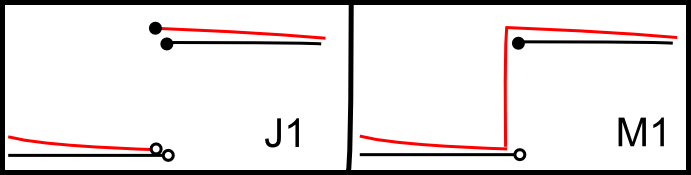
\includegraphics[width=.5\textwidth]{j1m1tops.png}
\caption{\textbf{Topologies for cadlag functions.} \textbf{Left:} Two functions that are ``close" in the J1 topology.  Note that the magnitude of their jumps are similar. \textbf{Right:} Two functions close in the M1 topology.  Jumps are not required to be close in this case, but rather the Hausdorff distances of each function's completed graph. }\label{j1m1}
\end{centering}
\end{figure}

Throughout this thesis, our focus will be on stochastic processes which are cadlag, or are right continuous with lefthand limits. Let $(\mathfrak M,d)$ denote a metric space with metric $d$.   In the following, we use the $J1$ Skorohod topology, denoted $\mathbb D([0,t],\mathfrak M)$. For our purposes, $\mathfrak M$ will either be $\mathbb{R}^+$ or  $\mathcal M(\mathbb{R}^+)$, the space of finite measures on $\mathbb{R}^+$ with the Prohorov metric \cite{billingsley2009convergence}.
The $J1$ topology  allows for convergence of functions that ``wiggle" in time as well as space, and has  the following characterization (see \cite{jac87}): 

Let $\mathscr R$ be the set of continuous reparameterizations $r: [0,t]\rightarrow \mathbb{R}^+$: functions that are strictly increasing, where $r(0) = 0$ and $r(t)=t$.  A sequence of functions $\alpha_n \rightarrow \alpha$ in $\mathbb{D}([0,t],\mathfrak M)$ if and only if there is a sequence $r_n \in \mathscr R$ with 

\begin{enumerate}
\item $\sup_s |r_n(s)-s| \rightarrow 0,$
\item $\sup_{s \le t} d(\alpha_n(r_n(s)), \alpha(s)) \rightarrow 0.$ 
\end{enumerate}
as $n \rightarrow \infty$. If $\alpha(t)$ is continuous, the functions actually converge in the local uniform topology. However, in general,  the local uniform topology is strictly stronger than the Skorohod J1 topology, but this fact won't be used, since limiting functions of our interest in this paper will have no jumps (see Remark \ref{unifremark}).  


